\edef\mychapter{Set Theory}
\edef\mychapterdate{June 18, 2024}

\chapter{\mychapter}
\section{Set Theory}
Often, in mathematics, we like to group abstract things, also known as a mathematical object, into sets. A mathematical object is, simply put, a \textit{thing} we like to talk about in math, such as functions, numbers, matrices, other sets, etc.
Although seemingly simple, these sets are incredibly powerful, so powerful in fact that most modern mathematics today is built off the backbones of set theory. 
For our purposes here, we only need a very elementary understanding of set theory, as a deeper dive, though fascinating, can be very confusing, difficult, and at times controversial.\footnote{This controversy mostly arises from the infamous \href{https://en.wikipedia.org/wiki/Axiom_of_choice}{axiom of choice}. 
Simply put, given any set of sets that are not empty, one can always find a way to way to map a child set to an element in that child set. Though seemingly simple, due to its complications with infinite sets, it has deep consequences in all mathematics and how we deal with infinities in the universe.}
\subsection{Notation}
Before we move any further, we should get some basic notation out of the way, below is a list of all of the important symbols that we will be using in this class:
\begin{center}
	\begin{longtable}{| c | m{6cm} |}
		\hline 
		Symbol & Meaning \\
		\hline 
		$\in,\notin$   & in and not in respectively. Typically to denote that an object belongs or doesn't belong to a set \\
		\hline 
		$\subset, \subseteq$ & proper subset, subset, we discuss the distinction later \\
		\hline
		$\not\subset, \not\subseteq$ & not a proper subset, or subset \\
		\hline
		$\setminus$ & Set difference \\
		\hline
		$=$ & two sets are equivalent to one another \\
		\hline 
		$\cup$ & Union \\
		\hline
		$\cap$ & Intersect \\
		\hline

		$\overline{A}$ & Compliment of set $A$ \\
		\hline
		$\{x : \phi(x)\}$ & Defines a new set using variable $x$ on the condition $\phi(x)$\\
		\hline
		$A=(a,b),[a,b]$ & Defines a set on the interval where for any $x$ $a < x < b$ or $a\le x \le b$ respectively, $x\in A$. \\
		\hline
		$\varnothing$ & empty set, a set with no elements \\
		\hline
	\end{longtable}
\end{center}

Of the following, let us first draw our attention to the idea of a subset. A subset, in most simple terms, is just a set that is entirely contained within a larger parent, as shown in figure \eqref{fig:subset}. 
\begin{figure}[h]
	\centering
	\resizebox{0.3\linewidth}{!}{
	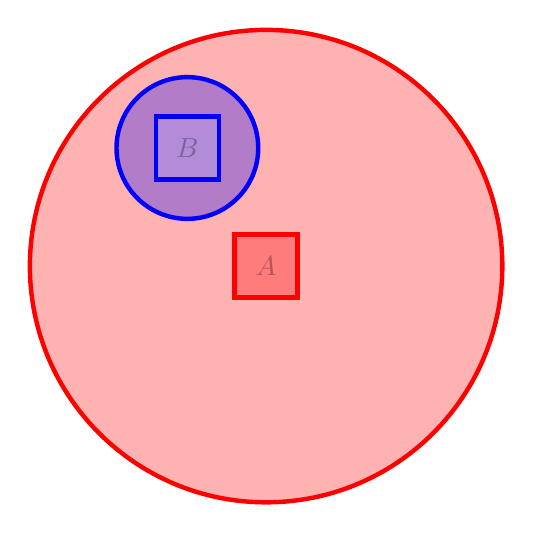
\begin{tikzpicture}
		\draw[ultra thick, draw=red, fill=red, fill opacity=.3] (0,0) circle (3)
			node[black,draw=red, fill=red, minimum size=0.8cm] {$A$};
		\draw[ultra thick, draw=blue, fill=blue, fill opacity=.3] (-1,1.5) circle (0.9)
			node[black,draw=blue, fill=blue!30, minimum size=0.8cm] {$B$};
	\end{tikzpicture}}
	\caption{Here we claim $B\subset A$}
	\label{fig:subset}
\end{figure}
As you may have noticed, I've decided to use $\subset$ as opposed to $\subseteq$ in the figure.
Although both would have been equally valid, I specifically chose the former to shed light on the fact the two sets $B$ and $A$ are not equal. 
Similar to $>$ and $\ge$, the line underneath simply implies the possibility that the subset is equal to the original set.\footnote{
It is important to note, however, that in certain texts, the distinction is not made between proper and non-proper subsets and the symbol $\subset$ is used for either case. In all my texts, I will be making this distinction, and $\subset$ will only refer to proper subsets.}

Now we have some basic intuition for this concept, let's shed some light on the rigorous definition of a subset, as such a definition will help us prove that a set is indeed a subset of another.
\begin{define}
	$A\subseteq B$ if and only if \footnotemark for every $a\in A$, $\in B$.
\end{define}
\footnotetext{If you're unfamiliar with the term \textit{if and only if}, when we say $A$ if and only if $B$, we imply if $A$ then $B$ and if $B$ then $A$, hence the implication goes both ways. Another way to say this is $B$ is \textit{necessary and sufficient} for $A$, or vice versa.}

With this definition, we can construct a definition of set equality.
In particular, when we say two sets are equal, we should expect that every element in one set should be in another and vice versa. In other words, we expect
$$a\in A \text{ if and only if } a \in B.$$
Therefore, a definition that would naturally follow is
\begin{define}
We say $A=B$ is and only if $A\subseteq B$ and $B\subseteq A$.\footnotemark
\end{define}
\footnotetext{As an exercise, try to prove this is equivalent to the characterization we gave before.}

The next symbol I'd like to focus on is the set difference. Very similar to subtraction, if we have two sets $A$ and $B$, $A\setminus B$ is simply defined as the set of elements that are in $A$, but not in $B$ as shown in figure \eqref{fig:diff}.
\begin{figure}[h]
\centering
\resizebox{0.3\linewidth}{!}{
	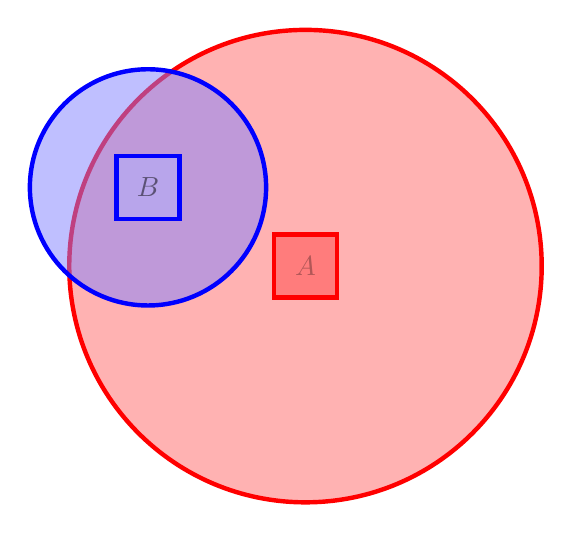
\begin{tikzpicture}
		\draw[ultra thick, draw=red, fill=red, fill opacity=.3] (0,0) circle (3)
			node[black,draw=red, fill=red, minimum size=0.8cm] {$A$};
		\draw[ultra thick, draw=blue, fill=blue!50, fill opacity=0.5] (-2,1) circle (1.5)
			node[black,draw=blue, fill=blue!30, minimum size=0.8cm] {$B$};
	\end{tikzpicture}}
	\caption{$A\setminus B$ defined in red}
	\label{fig:diff}
\end{figure}

We can also formalize this idea in a more formal definition.

\begin{define}
	$x\in A\setminus B$ if and only if $x\in A$ and $x\notin B$.
\end{define}


\subsection{Set Theory and Logic}
The idea of the intercept or union can be shown most clearly with a Venn diagram like in figure \eqref{fig:union}.
\begin{figure}[h]
\centering
\resizebox{0.6\linewidth}{!}{
	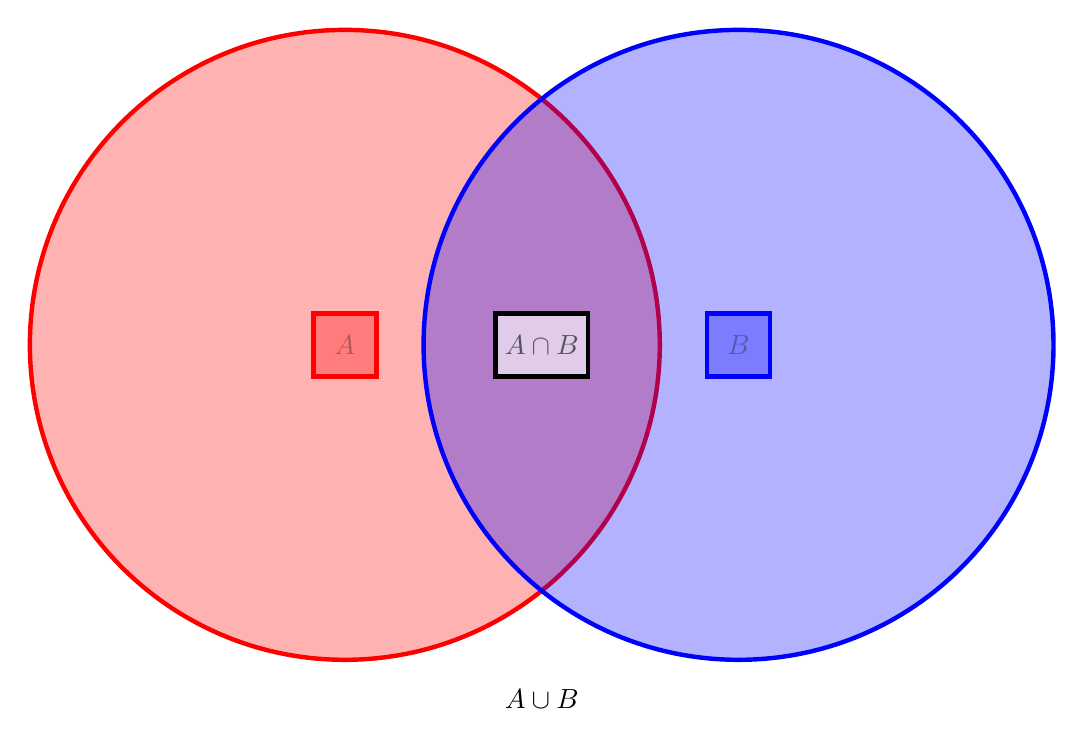
\begin{tikzpicture}
		\draw[ultra thick, draw=red, fill=red, fill opacity=.3] (-2.5,0) circle (4) node[black,draw=red, fill=red, minimum size=0.8cm] {$A$};
		\draw[ultra thick, draw=blue, fill=blue, fill opacity=.3] ( 2.5,0) circle (4) node[black, draw=blue, fill=blue, minimum size=0.8cm] {$B$};

		\draw (0,0) node[ultra thick, draw=black, fill=white, minimum size=0.8cm, fill opacity=0.6] {$A\cap B$} ;
		
		\draw (0,-4.5) node {$A\cup B$} ;
	\end{tikzpicture}}
	\caption{}
	\label{fig:union}
\end{figure}
From here, it is clear that when taking the union of the two sets, we are essentially \textit{adding} the two sets together, or other words, every element $x\in A\cup B$ is a member of either in $A$ \textbf{or} $B$.
An important note here is that a set doesn't contain duplicates of an object, therefore, when taking the union, an object is only included once in the output.

Then the intersect is the region where every element $x\in A\cap B$ is both in $A$ \textbf{and} $B$.\footnote{the intersect also bears stark resemblance with an elementary operation, which, as you may have assumed, is multiplication. 
We won't get into the details here, but just understand that it follows many of the same properties as multiplication}
I emphasize the "and" and "or" parts of the previous statements since I believe it's important to see the relationship between these very mathematical ideas and words we use in our everyday lives.\footnote{
It is important to note, however, that the or used in this case is slightly different from the or we use in everyday life.
This is because we tend to deal more with exclusive or, where the or we deal with in math is non-exclusive. 
If you have no idea what I'm talking about, then forget that you even read this section.}

Now, with this intuition of these operations, we can move on to rigorously define them as the following:
\begin{define}
$x\in A\cup B$ is and only if $x\in A$ or $x\in B$.	
\end{define}
\begin{define}
$x\in A\cap B$ is and only if $x\in A$ and $x\in B$.	
\end{define}

The complement of a set can be thought of exactly as the word \textbf{not}.
\begin{figure}[h]
\centering
	\resizebox{0.3\linewidth}{!}{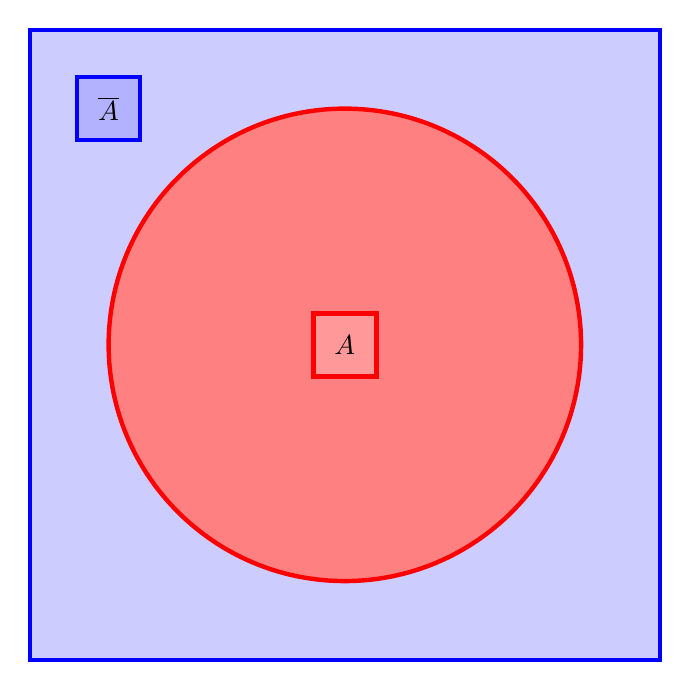
\begin{tikzpicture}
		\draw[ultra thick, draw=blue, fill=blue, fill opacity=.2] (-4,-4) rectangle (4,4);
		\draw[ultra thick, draw=red, fill=red!50] (0,0) circle (3) node[black,draw=red, fill=red!40, minimum size=0.8cm] {$A$};
		\draw (-3,3) node[ultra thick, black, draw=blue, fill=blue!30, minimum size=0.8cm] {$\overline A$};
	\end{tikzpicture}}
	\caption{If the entire square is $B$, then $\overline A, A\subseteq B$}
	\label{fig:not}
\end{figure}
We can generalize figure \eqref{fig:not} by saying that every $x\notin  A$ must be in $\overline A$.
It is important to note here that generally, when talking about a compliment, you need to know what you are "complementing" over, in essence, you must know what your set is a subset of.
Unless you go into more advanced mathematics, generally, you can assume that this will be the real numbers, or in more isolated cases, the set of complex numbers, but nothing more than that.
Now, formalizing our intuition gives the following definition:
\begin{define}
	Suppose $A\subseteq U$. Then $x\in \bar A$ if and only if $x\in U$ and $x\notin A$.\footnotemark
\end{define}
\footnotetext{Notice, we could have also defined $\bar A$ as $U\setminus A$, which has the advantage of specifying a global set which we are taking the compliment over.}

\subsection{Defining Sets}
The last two notations in the chart are simply ways in which we can define new sets. Let's say we are trying to define a set that consists of only points on the unit circle. So, in this case, we would be defining a set of ordered pairs. We first note that any point that lies on a circle satisfies
$$x^2+y^2=1.$$
Then, we can simply define $S$ as
$$S=\{(x,y) : x^2+y^2=1\}.$$
This might still seem confusing, but typically, colons in math can be read as \textit{such that} or \textit{given} hence the statement above is equivalent to saying: 
\textit{the set S is equivalent to the set of all real ordered pairs given they satisfy $x^2+y^2=1$}. 
This notation is known as set builder notation since, in essence, we are building a set based on a given set of conditions.
Sometimes, we like to be a bit more specific and explicitly declare that $(x,y)$ is an ordered pair and write
$$S=\{(x,y)\in \real^2 : x^2+y^2=1\}.$$
where $\real^2$ is the set of all real ordered paris.

We then draw our attention to an alternative way to define sets in real numbers, which is interval notation. Generally, in precalc, you will see this more often, as it is a quick and easy way to define a set on a given interval. Let's say we are trying to define a set $S$, where $S$ is the set of all reals between 2 and 5, excluding the values 2 and 5 (the endpoints). Then we write
$$S=(2,5).$$
Alternatively, we can change the parentheses to square brackets, where then we would have
$$S=[2,5]=\{x : 2 \le x \le 5\}.$$
We see here that where parentheses correspond to strict inequality, square brackets correspond to a non-strict inequality. We can also mix and match and define sets like
$$[1,5)=\{x : 1 \le x < 5\},$$
or we can use it in combination with the union and intersect to combine multiple intervals such that
$$[1,5)\cup (6,10]=\{x : 1 \le x < 5 \text{ or } 6 < x \le 10\},$$
or
$$[1,5)\cap (3,\infty)=\{x : 3 < x < 5\}.
\footnote{When we deal with infinity, always use $()$ since infinity is not in the real numbers, and hence we cannot include $\infty$ in our set.}$$

\subsection{Very Important Sets}
Certain sets in mathematics are so important that we give them a special symbol

\begin{center}
	\begin{longtable}{| c | m{6cm} |}
		\hline 
		Symbol & Definition \\
		\hline 
		$\integ$ & Set of all integers \\
		\hline
		$\nat$ & Set of all natural numbers \\ 
		\hline
		$\mathbb{W}$ & Set of all whole numbers \\
		\hline
		$\real$ & Set of all real numbers \\
		\hline
		$\complex$ & Set of all complex numbers \\
		\hline
		$\rat$ & Set of all rational numbers \\
		\hline
	\end{longtable}
\end{center}

Some of these, I hope, are very familiar to all of you, but I'd like to shed some light on $\nat$ and $\mathbb{W}$, as these might not be so familiar to many of you. The whole numbers are simply defined as positive real numbers, including 0 or
$$\mathbb{W}=\{x\in \integ : x\ge 0\}.$$
Then, the natural numbers are simply
$$\nat=\mathbb{W}\setminus\{0\},$$
or in other words, positive integers without 0.\footnote{In different countries, this might be defined differently, like in France, $\nat$ is defined in the same way as we defined the $\mathbb{W}$.}

\section{Proof by Induction}
\subsection{Well-Ordering Principle}
An important idea that I'd like to draw our attention to is the idea of a well-ordered set.
This might seem at first like a bunch of mathematical mumble jumble, but it has serious consequences when it comes to mathematical reasoning.
But before we get to the implications, let's first examine what exactly this well-ordering principle is. 

Let's start by looking at the natural numbers. Our first and most obvious observation is that the natural numbers are \textit{totally ordered},
meaning you can take any two elements of the set and declare one is larger than the other, given they are not equal. 
Then, looking further, we realize by taking any subset of the natural numbers, finite or infinite, as long as this set isn't empty, there must be a least element since no matter what is in any of these subsets, 1 is always less than everything, and if 1 isn't in the set, we go to 2 or 3, and the same logic applies. This is a well-ordered set; we take this as a defining property of natural numbers.\footnote{Rigoursly proving this fact $\nat$, using the formal definition of $\nat$ is very difficult and confusing.}
We can formalize our observation here and propose a definition for a well-ordered set:
\begin{define}
	Let $S$ be a set where for every $a,b\in S$, exactly one of
	$$a<b \jor a>b \jor a=b$$
	is true. Then $S$ is \textbf{well-ordered} if and only if for every $T\subseteq S$, there exists $x_l$ such that for every $x\in T$, $x_l\le x$.
\end{define}

It is important to note here that this property occurs in other types of sets other than just the natural numbers, as we will soon find, we can extend this idea to a set of ordered statements.

\begin{ex}
	We will demonstrate the well-ordered principle in this example. Let's use the set
	$$S:=\{2n: 2n>7, n\in\nat\}.$$
	It should be immediately clear that this is the set of positive even numbers greater than 7. Therefore, we conclude $S\subseteq \nat$.
	We can also check that $8$ is indeed the least element of $S$, i.e., for every $k\in S$, $8\le k$.
	
	Then, let's see why a set like $\integ$ is not well-ordered. Suppose
	$$T:=\{n:2n,n\in \integ\}.$$
	It should be clear that $T$ is the set of all even numbers, positive or negative.
	Since for every element $k\in T$, we can find a smaller even number, we conclude that $T$ cannot have the least element.
	Since the well-ordering principle requires that any arbitrary subset has a least element, we have $\integ$ is not well-ordered.
\end{ex}

\subsection{Example of Proof by Induction}
This may or may not be a new idea for some, but first, I will attempt to demonstrate the power of proof by induction by proving a very simple statement.
\begin{ex}
In the following example, I'd like to show for a sequence $1,2,3,...,n$, where $n\in\nat$, the sum is exactly
$$\frac{n(n+1)}{2}.$$
First, let's check that our formula works by checking against a sequence with $n=1$. We find the sum is 1 and
$$\frac{1(1+1)}{2}=1$$
hence verifying our formula works for $n=1$. Let's call this case, where $n=1$ is the base case.
We can keep checking for $n=2,3,4...$, but since we want to know that this formula works for all possible $n$, this is a never-ending process, thereby making it impossible to construct a rigorous proof.
This means we must look for another technique to prove our desired statement. Let's suppose, for a minute, that for some $m\in\nat$, our formula produces the right result. Then, using our assumption, we claim that
$$1+2+...+m+m+1=(1+2+...+m)+m+1=\frac{m(m+1)}{2}+m+1$$
Then, by manipulating the expression, we get
$$\frac{m(m+1)}{2}+m+1=\frac{m(m+1)+2(m+1)}{2}=\frac{m^2+m+2m+1}{2}$$
$$=\frac{m^2+3m+1}{2}=\frac{(m+1)(m+2)}{2}=\frac{(m+1)([m+1]+1)}{2}$$
which is exactly the expression we would get if we substituted $m+1$ into our formula. Therefore, we have proven if the formula is true for $m$, then it must be true for $m+1$. Let's call this part the inductive step.
Here, I claim, without proof, that the base case, in combination with the inductive step, proves by induction that our formula works for all $n$.
But a question remains: how exactly am I able to make such a bold conclusion?\footnote{
Philosophically speaking, in general everyday life, inductive reasoning is inherently flawed since your conclusions rely on possibly flawed assumptions about the past. 
In math, we only accept statements as true if we can deduce them from other true statements, which contradicts what we've done here since we did exactly what I said was inherently flawed.
But somehow, math has a way of deductively proving that what I did here, in fact, is okay.}
\end{ex}

\subsection{Proof of Induction by Deduction}
This brings us back to the well-ordered principle.
First, we need to organize all of our statements into a set.
This idea might seem quite unnatural, but if you think about our statements as functions that take in a natural number and output a true or false, this idea comes very naturally since we know we can organize functions into a set.
As in our previous example, take for instance the statement \textbf{$1+2+...+n$ is equal to $\frac{n(n+1)}{2}$} as a function of $n$, called $P(n)$, where $n$ is any natural number, we now know that $P(n)$ is true for every $n$, hence the statements $P(1),P(2),P(3),...$ are all true. 
We can make another example of this idea: suppose we define a statement $Q(n)$ as \textbf{$n$ is odd}. Then we can define a set $S=\{Q(n):n\in\nat\}$. Then we know $Q(1),Q(3),Q(5),...$ is true and $Q(2),Q(4),Q(6),...$ is obviously false. Now equipt with this, we will attempt to prove our first lemma:
\begin{lemma}
\label{lem:well-order}
	Let $P(n)$ be an arbitrary statement with argument $n\in\nat$. If
	$$S:=\{P(n):n\in\nat\},$$
	then $S$ is well-ordered.
\end{lemma}
\begin{proof}
	We will attempt to prove this proposition with the help of figure \eqref{fig:induct:map}.
	\begin{figure}[h]
	\centering
		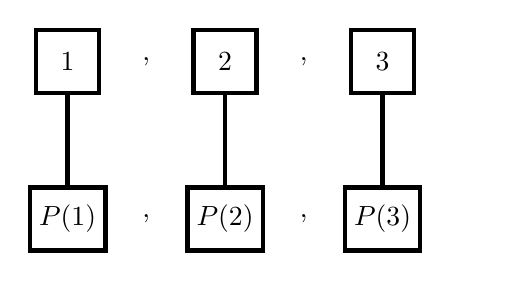
\begin{tikzpicture}
			\draw[ultra thick,->] (-2.5, 1) node[ultra thick, black,draw=black, fill=white,minimum size=0.8cm] {1}
			-- (-2.5,-1) 
			node[ultra thick, black,draw=black, fill=white,minimum size=0.8cm] {$P(1)$};
			\draw (-1.5,1) node {,};
			\draw (-1.5,-1) node {,};
			
			\draw[ultra thick,->] (-0.5, 1) node[ultra thick, black,draw=black, fill=white,minimum size=0.8cm] {2}-- (-0.5,-1)
			node[ultra thick, black,draw=black, fill=white,minimum size=0.8cm] {$P(2)$};
			\draw (0.5,1) node {,};
			\draw (0.5,-1) node {,};
			
			\draw[ultra thick,->] (1.5, 1) node[ultra thick, black,draw=black, fill=white,minimum size=0.8cm] {3}-- (1.5,-1)
			node[ultra thick, black,draw=black, fill=white,minimum size=0.8cm] {$P(3)$};
			
			\draw (2.7, 1) node{$\hdots$};
			\draw (2.7, -1) node{$\hdots$};
		\end{tikzpicture}
		\caption{}
		\label{fig:induct:map}
	\end{figure}
	As shown in the diagram, we can map every natural number to a unique statement and vice versa.
	Then we can define an ordering on $S$ such that for any $P(m_1),P(m_2)\in S$, $P(m_1)<P(m_2)$ if and only if $m_1<m_2$.
	Therefore, for any $T\subseteq S$.
	Then we can construct
	$$N:=\{n\in \nat: P(n)\in T\}$$
	Then, we have $N\subseteq \nat$ implying $N$ has a least element. Let $n_l$ be the least element of $N$.
	Then, since $P(n_l)\in T$ by definition, we claim this is the least element of $T$.
	To show this is indeed the least element, consider any $P(m)\in T$. By definition of $N$, we have $m\in N$. Therefore $n_l\le m$, implying $P(n_l)\le P(m)$ thereby completing the proof.
\end{proof}

\begin{theorem}[Induction]
	Suppose $P(n)$ is some arbitrary statement that depends on $n$. Then if
	\begin{enumerate}
		\item $P(1)$ is true (Base case)
		\item If $P(n)$ is true, then $P(n+1)$ is true. (Inductive step)
	\end{enumerate}
	Then $P(n)$ is true for all $n$.
\end{theorem}
\begin{proof}
	This proof will be by contradiction. First, assume there exists $P(n)$ that satisfies the above conditions, where for some $k\in\nat$, $P(k)$ is false. 
	Then define 
	$$S=\{P(n):n\in\nat\}.$$
	Then let
	$$F:=\{P(n)\in S: P(n)\equiv \text{false}\}.$$
	Then we have $F\subseteq S$.
	Then by our assumption, $P(k)\in F$ hence $F\neq \varnothing$.
	Since $S$ is well-ordered by lemma \eqref{lem:well-order}, $F$ must have a least element $P(n_l)$. 
	$n_l\neq 1$, since by assumption $P(1)$ is true.
	Therefore, $P(n_l-1)\in S$. 
	But $P(n_l-1)\notin F$, since $P(n_l-1)<P(n_l)$, implies $P(n_l-1)$ is true.
	This means $P(n_l)$ must also be true by the inductive step assumption.
	This is a contradiction of our original assumption, hence $F\equiv \varnothing$. 
	This concludes our proof of induction.
\end{proof}

To summarize, if we can simply prove that some base case $P(b)$ is true, by then proving that $P(n)$ being true implies $P(n+1)$ is true, we can confidently claim that for every $n\ge b$, $P(n)$ is true.
\subsection{More Examples}
\begin{ex}
	In this example, we'd like to prove $9^n-1$ is divisible by $8$ for all $n\in\mathbb{W}$. 
	To begin, we'd first like to prove that the base case is true, and in this case, the base case is $n=0$.\footnote{For the base case, $n$ does not necessarily have to be 0, but the index of the base case is the least that is guaranteed to be true with our current approach at induction (try to prove this fact by modifying the above proof).} Since
	$$9^0-1=0$$
	is divisible by 8, we can establish that our base case is true. Then, assume the statement is true for some arbitrary $k$. Then there exists, by the definition of divisibility, some $m\in\integ$ such that
	$$9^k-1=8m$$
	which implies
	$$9^k=8m+1$$
	Then for $k+1$,
	$$9^{k+1}-1=9(9^k)-1=9(8m+1)-1$$
	$$=72m-8=8(9m-1)$$
	Since $8(9m-1)\in\integ$, this implies $9^{k+1}-1$ is divisible by 8. Therefore, by induction for all $n\in\mathbb{W}$, $9^n-1$ is divisible by 8.
\end{ex}

\begin{ex}
	In this example, we'd like to prove $n^2<2^{n+1}$ for any $n\in\nat$. This will be a little less straightforward than in our previous examples, but what is the same is proving the base case is true, which is trivial by substitution of 1 for $n$. For our inductive step, we assume for some $k$, $k^2<2^{k+1}$.
	Then
	$$2^{k+2}=2\cdot 2^{k+1}>k^2+2^{k+1}.$$
	If we notice, what we want on the right side is 
	$$(k+1)^2=k^2+2k+1.$$
	Somehow, we must convert the $2^{k+1}$ to $2k+1$. We could do this by proving 
	$$2^{k+1}>2k+1$$ 
	for all $k\in\nat$, which 
	$$2^{k+2}>(k+1)^2$$ 
	would immediately follow.
	To prove the previous statement, we leverage induction again. By substituting $k=1$, we find the base case is trivial. Then, for our inductive step, we let be $m\in\nat$ such that $2^{m+1}>2m+1$.
	Then
	$$2^{m+2}=2\cdot2^{m+1}>2(2m+1)=2m+2m+2.$$
	Since $m\ge 1$,
	$$2m+2m+2>2m+4>2m+2+1=2(m+1)+1.$$
	Therefore, by induction, we conclude 
	$$2^{k+1}>2k+1$$
	hence
	$$2^{k+2}>k^2+2^{k+1}>k^2+2k+1=(k+1)^2.$$
	Therefore, by induction, we claim $n^2<2^{n+1}$.
\end{ex}

\section{Exercises}
1. Let $A=\{1,\beta,20\}$, $B=\{\text{two},\beta,20\},C=\{20,\text{one},\alpha\}$. Give the sets resulting from
\begin{enumerate}[label=\alph*)]
	\item $A \cup B$
	\item $A \cap B$
	\item $C \setminus A$
	\item $A \cup (B\cap C)$
\end{enumerate}

\noindent
2. Define each of the following sets in set builder notation.
\begin{enumerate}[label=\alph*)]
	\item The interval $-5<x<3$ or $-10<x<-3$.
	\item The set of all even numbers.
	\item The set of all positive perfect squares (excluding 0).
\end{enumerate}

\noindent
3. Let $q$ be any real number such that $q\neq1$. Show, for any $n\in\nat$,
$$\sum_{k=1}^nq^k=\frac{q^{n+1}-q}{q-1}.$$
(Hint: If you've never seen the summation notation, $\sum_{k=1}^nq^k=q+q^2+...+q^n$.)

\noindent
4. Prove $5^n+5<5^{n+1}$ for all $n\in\nat$.

\noindent
5. \textbf{(Challenge)}. For any statement, $P(n)$ for $n\in\nat$, suppose 
\begin{enumerate}
	\item $P(1)$ is true
	\item For $n\in\nat$, $P(n)$ implies $P(n+2)$
\end{enumerate}
Prove $P(n)$ is true for every positive odd integer. 









